
The majority of DP-SGD techniques assume a fixed privacy requirement (i.e., budget $\varepsilon$) for all data contributors, and focus on various adaptations of learning rate or budget consumption throughout the learning process to improve the privacy-accuracy trade-off (see Section~\ref{sec:adaptation}). The privacy budget used in the training must adhere to the most stringent privacy requirement among all data contributors. However, in practice, various data contributors may have differing privacy expectations~\cite{userConc}. Data points from contributors with lower privacy requirements could potentially offer more valuable information for training machine learning models. Consequently, setting a uniform privacy budget across all data points may unnecessarily lower the training accuracy.

Recently~\cite{ipate}, a novel research direction has surfaced, which focuses on supporting the enforcement of heterogeneous privacy constraints across the training dataset. Data points are partitioned into several groups, each with its own privacy budget. Essentially, the concept involves allocating greater privacy budgets to less sensitive data points and lower budgets to more sensitive ones. In this section, we review the several approaches for {\em individualized} privacy budget assignment.

The idea of individualized privacy constraints has been considered in the differential privacy literature even before DP-SGD emerged, in the context of statistical queries. The early work by Jorgensen et. al. \cite{Jorgensen2015} proposed two directions. The first one involves a two-step process: non-uniform sampling based on each tuple's specific privacy requirements, followed by applying a differentially private mechanism to the sampled dataset. This method effectively combines randomness from both steps to achieve personalized privacy guarantees. The second approach, inspired by the exponential mechanism developed by McSherry and Talwar \cite{mcsherry2007mechanism}, offers a more direct route to achieving Personalized Differential Privacy (PDP). 

Later on, the work done by Li et. al. \cite{li2017partitioning} explored two partitioning methods aimed at achieving PDP while optimizing individuals' privacy budgets and enhancing utility. These methods, termed {\em privacy-aware} and {\em utility-based} partitioning, group records with diverse privacy budgets into different bins. Each bin undergoes DP aggregate computation using its minimum privacy budget, and the perturbed results are aggregated in the final output.

A recent study \cite{Niu2021} took an adaptive approach to PDP. The proposed adaptive framework for personalized differential privacy ({\em AdaPDP}) dynamically selects noise generation algorithms and determines parameters such as sensitivity and noise magnitude based on query functions, data distributions, and privacy settings, in order to maximize data utility. Additionally, AdaPDP conducts multiple rounds of utility-aware sampling to meet diverse privacy requirements for individual users.

Most studies emphasize two key directions to achieve individualized privacy: {\em sampling} and {\em grouping}. In the former approach, sampling probabilities are assigned to data points inversely proportional to their privacy concerns, ensuring that records with higher privacy demand are sampled less frequently. In the latter, points with equal privacy concerns are clustered together, with higher-privacy groups undergoing more noise addition than lower concern groups. Figure~\ref{sampleGroup} illustrates the two approaches.

\begin{figure}[h]
\centering
    \subfloat [Sampling\label{fig:subfigA}] {
        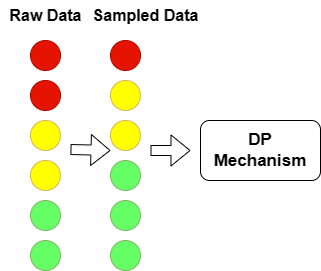
\includegraphics[width=0.4\linewidth]{submissions/submission5/figs/sample.png}}
    \subfloat[Grouping\label{fig:subfigB}]{
          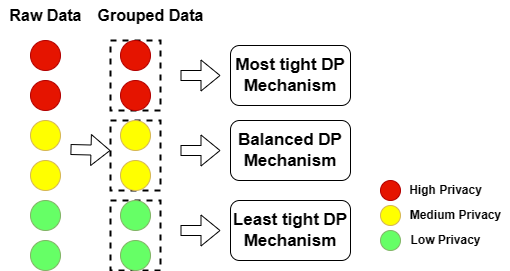
\includegraphics[width=0.6\linewidth]{submissions/submission5/figs/grouped.png}}    
   
   \caption{Sampling Approach vs Grouping Approach}\label{FigDiff}
   \label{sampleGroup}
\end{figure} 

%In the upcoming lines we are going to discuss different approaches that adapted the same concept for the differentially private deep learning.

The \textbf{upsampling} approach is a technique introduced in~\cite{ipate} in conjunction with the Private Aggregation of Teacher Ensembles (PATE) algorithm. PATE is an alternative to DP-SGD for training machine learning models on sensitive data while preserving individual privacy. It involves training multiple teacher models on disjoint subsets of the data, aggregating their predictions with differential privacy, and then training a student model using the noisy aggregated labels. PATE allows for effective model training while ensuring privacy protection, making it suitable for various applications in fields like healthcare and finance~\cite{pate}.

The upsampling mechanism relies on duplicating sensitive data
such that overlapping data-subsets can be allocated to different teachers. Thereby, data with higher privacy budgets are used to train a
higher number of teachers, thus revealing more information from data points with less restrictive privacy needs, and restricting the level of information derived from points with higher demands~\cite{ipate}. The algorithm ensures that points are duplicated by an integer according to the privacy budget ratios. Algorithm~\ref{algo:algPATE} shows how the upsampling factor is calculated for each data point.

\begin{algorithm}[H]
\SetAlgoLined
\KwIn{Privacy budgets $\{ \varepsilon_d \}$ for each data point $d$, precision $p \in \mathbb{N}$}
\KwOut{Upsampling factor $u_d$ for each data point $d$}
{ $\{ \varepsilon_1, \ldots, \varepsilon_j \} \leftarrow \text{unique}(\{ \varepsilon_d \})$ } \tcp*{Get unique budgets}
\For{each $\varepsilon_j$}{
    $\bar{\varepsilon}_j \leftarrow \varepsilon_j \cdot 10^p$ \tcp*{Upscale budgets}
}
$D \leftarrow \text{Greatest Common Divisor}(\bar{\varepsilon}_1, \ldots, \bar{\varepsilon}_G )$; \\
\For{each $\bar{\varepsilon}_j$}{
    $u_d \leftarrow \frac{\bar{\varepsilon}_j}{D}$; \\
}
\caption{Upsampling method in PATE~\cite{ipate}}
\label{algo:algPATE}
\end{algorithm}

Using the same upsampling technique, the work in~\cite{haveit} proposed a method that relies on sampling data points with different sample rates ${q_1, . . . , q_P }$ depending on their individual privacy budgets. In this case, the noise multiplier $\sigma_{sample}$ is fixed. Data points with higher privacy budgets (weaker privacy requirements) are assigned higher sampling rates than those with lower privacy budgets. This modifies the Poisson sampling process for DP-SGD to sample data points with higher privacy budgets within more training iterations.
Using the minimum privacy budget of $\epsilon_1$, the algorithm begins by initializing the $\sigma_{sample}$ with $\sigma$ from conventional DP-SGD, which is the noise multiplier needed for the privacy group $G_1$, which has the strongest privacy requirement of all groups. This is equivalent to instantiating $\sigma_{sample}$ using the overall privacy groups' upper bound noise. Next, they employ a $getSampleRate$ function to determine the sample rates for the specified privacy parameters. The algorithm then reduces $\sigma_{sample}$ repeatedly by a scaling factor that is marginally smaller than $1$, and  recalculates ${q_1,...,q_P}$ until their weighted average approaches $q$ (the traditional unified sampling rate).

The \textbf{grouping} approach is another technique used for individualized privacy budget assignment, which clusters together training examples with similar privacy requirements. In PATE, this step takes the form of a {\em weighting mechanism}~\cite{ipate} which adjusts how the aggregation of teacher votes is performed. It does this by assigning higher or lower weights to individual teachers' votes based on the privacy requirements of their training data points. Consequently, data points with similar privacy budgets $\varepsilon_j$, referred to as a privacy group $g_j$, must be assigned to the same teacher(s). Algorithm~\ref{algo:algPATE2} outlines the process of assigning weights $w_i$ to the teachers.

\begin{algorithm}[H] 
\SetAlgoLined
\KwIn{Privacy budget $\varepsilon_j$ and number of teachers $n_j$ for each privacy group дj, $j \in \{1, \ldots, G\}$, and total number of teachers $k$}
\KwOut{Weight $w_i$ for each teacher $t_i$}
$E \leftarrow \sum_{j=1}^{G} \varepsilon_j$; \\
\For{each privacy group $g_j$}{
    $\bar{\varepsilon}_j \leftarrow \frac{\varepsilon_j}{E}$ \tcp*{Relative privacy budget}
    $\bar{n}_j \leftarrow \frac{n_j}{k}$ \tcp*{Relative group size}
    $\bar{w}_j \leftarrow \bar{\varepsilon}_j \cdot \bar{n}_j$ ; \\
}
$W \leftarrow \sum_{j=1}^{G} \bar{w}_j$; \\
\For{each privacy group $g_j$}{
    $w_j \leftarrow \frac{\bar{w}_j}{W} \cdot k$ \tcp*{Make sum of weights match $k$}
    \For{each teacher $t_i$ with data from дj}{
        $w_i \leftarrow w_j$; \\
    }
}
%\caption{Assign weights to teacher models in the weighting method ~\cite{ipate}}
\caption{Weighting mechanism in~\cite{ipate}}
\label{algo:algPATE2}
\end{algorithm}

Based on grouping, the work in~\cite{haveit} proposes a {\bf scaling} method that adjusts the noise added to each gradient based on the privacy constraint of each data point. Current implementations of DP-SGD typically add noise to the sum of per-example clipped gradients over an entire mini-batch, resulting in the same amount of noise being added to all gradients. Instead, the authors of~\cite{haveit} introduce individualized clipping bounds ${c_1, ..., c_P}$ for each privacy level, effectively adjusting the scale of noise added on a per-example basis by modifying the sensitivity (clipping bound) of each example with a multiplier. Data points with higher privacy budgets (weaker privacy requirements) receive lower noise and higher clipping norms. As indicated in Equation~(\ref{eq:epsilon_bound}) below, the clipping bound $c$ does not directly impact the obtained $\varepsilon$; instead, the individualized privacy in the {\bf scaling} approach results from the individual noise multipliers ${\sigma_1, ..., \sigma_P}$. The privacy guarantee $\varepsilon$ depends on noise multiplier $\sigma$, sample rate $q$, the number of training iterations $I$, and the RDP order $\alpha$~\cite{haveit}. This translates into utility gains thanks to the overall increase in the signal-to-noise ratio during training.

\begin{equation}\label{eq:epsilon_bound}
\varepsilon \leq I \cdot 2q^2 \frac{{}\alpha}{\sigma^2}
\end{equation}

However, directly implementing individual noise multipliers per privacy group in {\bf scaling}  degrades training performance, because noise is added per mini-batch, while sampling and gradient clipping are performed per data point in DP-SGD. Restricting mini-batches to contain only data points from the same privacy group, which share the same noise multiplier, would lead to a loss of gains in the privacy-utility trade-offs resulting from subsampling. Therefore, while relying on mini-batches that contain data points with different privacy requirements (i.e., different noise multipliers), one can  specify a single fixed noise multiplier $\sigma$ scale.

To overcome this limitation, the work in~\cite{haveit} does not set noise multipliers ${\sigma_1, ..., \sigma_P}$ directly, but instead obtains them indirectly through individualized clipping bounds ${c_1, ..., c_P}$. In conventional DP-SGD, a gradient clipped to $c$ obtains noise with standard deviation $\sigma*c$. In the {\bf scaling} approach, gradients are clipped to $c_p = s_p*c$ with a per-privacy group scaling factor $s_p$, obtaining noise multiplier $\sigma_p c_p$. Noise is added according to $\sigma_{scale}c$ to all mini-batches. Thus, the effective noise scale $\sigma_p$ of each data point becomes $\sigma_p = \frac{1}{s_p} * \sigma_{scale}$. Data points with higher privacy budgets have $s_p > 1$, receiving lower noise multipliers, and vice- versa for lower privacy budgets.

Assuming all users in the training dataset have equal privacy concerns, certain training examples contribute more significantly to the learning process than others. This discrepancy means that some examples may pose higher privacy risks than others. A recent study by~\cite{individAccnt} introduces a novel approach to privacy assurance termed {\em output-specific individual differential privacy}. This method is designed to analyze the privacy guarantees of individual data points within models trained using DP-SGD. Investigations from~\cite{individAccnt} reveal that many data points benefit from stronger privacy guarantees than initially anticipated under the worst-case scenario, and that there is a robust correlation between a data point's privacy level and its associated training loss.

The fundamental concept behind output-specific $(\epsilon, \delta)$-DP involves defining the privacy parameter $\epsilon$ as a function of both the outputs and the specific target data point. In essence, for a given data point $d$ and a subset of outcomes $A \subset O$, an algorithm $A : D \rightarrow O$ satisfies output-specific individual $(\epsilon(A, d), \delta)$-DP for $d$ at $A$ if certain predefined conditions are met. To operationalize this approach, an algorithm is introduced to compute per-step RDP for each example using estimated individual gradient norms. Additionally, this algorithm facilitates the updating of individual gradient norms and the accumulated RDP. Furthermore, to streamline the computational cost associated with individual privacy assessment, two parameters are introduced: the frequency $K$ for computing batch gradient norms and the decision of whether to round individual gradient norms using a small constant $r$.